% WACV 2027 Paper Template
\documentclass[10pt,twocolumn,letterpaper]{article}

\usepackage[review,algorithms]{wacv}

% Additional packages needed beyond what wacv.sty already loads
\usepackage{multirow}
\usepackage{mathtools}
\usepackage{amsthm}

\definecolor{wacvblue}{rgb}{0.21,0.49,0.74}
\usepackage[pagebackref,breaklinks,colorlinks,allcolors=wacvblue]{hyperref}

\def\wacvPaperID{*****}
\def\confName{WACV}
\def\confYear{2027}

% ---- theorem environments ----
\newtheorem{proposition}{Proposition}
\newtheorem{remark}{Remark}
\theoremstyle{definition}
\newtheorem{definition}{Definition}

% ---- shortcuts ----
\newcommand{\Rhat}{\widehat{R}}
\newcommand{\Sigmay}{\Sigma_{y}}
\newcommand{\bc}{\boldsymbol{\mu}_c}
\newcommand{\sigc}{\boldsymbol{\sigma}_c^{2}}
\DeclareMathOperator*{\argmax}{arg\,max}

\title{FedCoP: Federated Co-occurrence-aware Prototypes for Multi-Label Medical Image Classification}

\author{Anonymous WACV submission\\
Paper ID \wacvPaperID}
% Note: authors will be added in camera-ready version

\begin{document}
\maketitle

% =====================================================================
\begin{abstract}
Federated prototype learning enables hospitals to train shared models without exchanging patient data by sharing class prototypes. However, existing methods model each pathology with an independent prototype and decode labels with independent per-class sigmoids---equivalent to assuming labels are conditionally independent given features. This assumption is clinically wrong for multi-label medical imaging where diseases co-occur as a matter of physiology (e.g., pleural effusion with atelectasis). We identify a structural reason this assumption fails under realistic federated settings: when each hospital sees only a subset of classes, no single client observes the global co-occurrence structure, as unseen-class entries are exactly zero rather than merely noisy.

We propose \textbf{FedCoP}, which augments distributional prototypes with a federatedly estimated co-occurrence correlation matrix $\Rhat$ and uses it on both sides of the pipeline: a structure loss $L_{co}$ aligning prototype geometry to $\Rhat$, and a mean-field decoder propagating evidence across co-occurring classes. $\Rhat$ is estimated from privacy-safe label sufficient statistics via count-weighted, de-biased fusion. We prove two results: (i)~the independent decoder is Bayes-optimal only under conditional independence, with regret $\Omega(\|\Sigmay-I\|_F^{2})$ that the mean-field decoder reduces; (ii)~the federated estimator is unbiased under participation reweighting, concentrates at rate $\tilde O(\sqrt{\log C/(K n_{\min})})$, and is unrecoverable by any single client under non-IID partitioning. Experiments on NIH ChestX-ray14 and MuReD under non-IID federated splits show consistent gains, with comprehensive ablations isolating each component.
\end{abstract}

% =====================================================================
\section{Introduction}

Chest radiography is the most frequently performed imaging exam, and reading a film is naturally multi-label: a single image often carries several findings at once, reflecting physiology (e.g., pleural effusion and atelectasis co-occur because fluid compresses lung tissue). A model that reads a chest film as fourteen independent questions is, clinically, reading it wrong. When such models are trained across hospitals under privacy constraints---the federated setting medicine requires---existing methods still treat pathologies as independent. This paper addresses that gap.

\subsection{Prototype-based FL and the independence assumption}

Federated learning trains shared models across hospitals without data exchange~\cite{mcmahan2017fedavg}. \textbf{FedProto}~\cite{tan2022fedproto} replaced weight sharing with prototype sharing: clients upload per-class mean feature vectors and the server averages them, while clients regularize local features toward global prototypes. This is communication-efficient, architecture-agnostic, and friendlier to privacy than sharing raw weights. Follow-up work strengthened prototype \emph{representation} (Gaussian mixture heads~\cite{zhang2024fedgmkd}, distributional heads) and \emph{aggregation} (quality-weighted fusion~\cite{zhang2024fedgmkd}, Bayesian fusion~\cite{chen2021fedbe}).

Yet every method in this line retains two independence assumptions harmful in multi-label medical imaging: (1)~\emph{Storage and alignment independence}: prototypes are stored as independent per-class objects with alignment losses treating classes in isolation. (2)~\emph{Decoding independence}: inference computes $p(y_c{=}1\mid \mathbf{x})=\sigma(-d_c/T)$ independently per class. Both faces assume labels are conditionally independent given features. In a domain where comorbidity is the norm, this is wrong, and we prove it is provably suboptimal (Sec.~\ref{sec:theory}).

\subsection{The federated co-occurrence opportunity}

Modeling label correlation runs into an immediate federated obstacle. Under realistic non-IID class partitioning, each hospital sees only $\text{ways}<C$ pathologies; a specialist center for effusion does not see enough hernia cases to know how the two relate. A client's co-occurrence count matrix $\mathbf{M}_k$ has zero rows/columns for every class it never sees---entries for unseen pairs are exactly zero, not merely noisy. No local data distinguishes ``these never co-occur'' from ``I never see these.''

This is a structural fact: the global $C{\times}C$ co-occurrence structure is recoverable only by federated aggregation of per-client sufficient statistics across clients whose class supports jointly cover all $C$ classes. Co-occurrence is therefore a \emph{structurally federated quantity}, invisible to any participant and visible only to the federation. The same necessity was observed by FedALC~\cite{an2024fedalc} in the single-positive-label setting; our contribution is what follows: a general sufficient-statistic estimator with de-biasing and concentration guarantees (Prop.~\ref{prop:estimation}), and its use on \emph{both} prototype geometry and decoding.

Four heterogeneity axes accompany the class-support gap, each making a different global quantity invisible to any single client: marginal prevalence varies across hospitals; co-occurrence structure itself varies with case mix; and participation is unequal. All share the same shape: a global quantity observed through biased local fragments, recoverable only by aggregation that corrects for bias.

\subsection{Contributions}

\begin{enumerate}
  \item \textbf{Federated co-occurrence structure.} A privacy-safe, count-weighted estimator of $\Rhat$ from label sufficient statistics $(\mathbf{m}_k,\mathbf{M}_k,n_k)$, with $\phi$-correlation de-biasing, shrinkage, and EMA smoothing. Unbiased under reweighted participation; concentrates at $\tilde O(\sqrt{\log C/(K n_{\min})})$.
  \item \textbf{Correlation-aware prototypes.} A structure loss $L_{co}$ aligning prototype cosine Gram to $\Rhat$, and a mean-field decoder using $\Rhat$, replacing heuristic contrastive/adversarial regularizers of prior FL with a single label-statistics-driven mechanism.
  \item \textbf{Theory.} Decoder-regret bound (mean-field never worse than independent sigmoids); federated-estimation theorem (unbiasedness, matrix-Bernstein concentration, single-client non-recoverability).
  \item \textbf{Minimal method and stronger evaluation.} A four-loss objective; full multi-label metrics (macro/micro AUROC, F1, Hamming, subset accuracy); comprehensive ablations isolating the federated structure, $L_{co}$, decoder, and six supplementary choices.
\end{enumerate}

% =====================================================================
\section{Related Work}

All methods below use an ImageNet-pretrained ResNet-50 backbone~\cite{he2016resnet} for fair comparison.

\noindent\textbf{Weight-sharing FL.} FedAvg~\cite{mcmahan2017fedavg} averages local SGD parameters. FedProx~\cite{li2020fedprox} adds a proximal term to curb client drift. FedBN~\cite{li2021fedbn} keeps BN statistics local for feature-shift non-IID. We use FedAvg and FedProx as weight-sharing baselines.

\noindent\textbf{Prototype-sharing FL.} FedProto~\cite{tan2022fedproto} shares point prototypes and is our direct baseline. FedGMKD~\cite{zhang2024fedgmkd} fits Gaussian-mixture prototypes by EM with discrepancy-aware aggregation; our re-implementation uses diagonal GMM with $K{=}3$ components, omitting the original's CKF distillation. FedBE~\cite{chen2021fedbe} applies Bayesian ensembling, which our precision-weighted fusion belongs to. FedSeProto~\cite{fedseproto2024} separates semantic/domain features with HSIC.

\noindent\textbf{Federated multi-label methods.} FedALC~\cite{an2024fedalc} estimates label correlations via per-instance label sets under single-positive labels, observing that co-occurrence is recoverable only through cross-client aggregation---the closest prior work. FedCoP differs in five ways: (i)~de-biased $\phi$-correlation from count statistics rather than hashed label sets; (ii)~distributional prototypes with Bayesian fusion; (iii)~$\Rhat$ shapes prototype \emph{geometry} via $L_{co}$; (iv)~mean-field decoder propagates evidence across co-occurring classes; (v)~formal decoder-regret bound and estimation theorem. FedMLP~\cite{sun2024fedmlp} addresses label missingness via pseudo-labeling and distillation---complementary along the label-completeness axis.

\noindent\textbf{Centralized multi-label.} Classifier chains~\cite{read2011classifier} and ML-$k$NN~\cite{zhang2007mlknn} model label dependence but cannot recover it under non-IID class partitioning---the federated gap FedCoP fills. Dembczy\'nski~\etal~\cite{dembczynski2012labeldependence} analyze when label dependence matters for loss minimization, motivating our Prop.~\ref{prop:regret}.

% =====================================================================
\section{Method: FedCoP}

FedCoP has one new component, the federated co-occurrence matrix $\Rhat$, and several inherited from prior prototype-FL and retained because they work. Per-class geometry (means and variances) stays in distributional prototypes (Sec.~\ref{sec:protos}); cross-class geometry (how classes relate) lives entirely in $\Rhat$. Training aligns prototype directions to $\Rhat$ (Sec.~\ref{sec:lco}); inference propagates evidence along it (Sec.~\ref{sec:decoder}). They are not redundant---they act on different objects, and ablations separate their contributions.

\subsection{Distributional prototypes}
\label{sec:protos}

Each class $c$ is modeled as a diagonal Gaussian $\mathcal{N}(\bc,\mathrm{diag}(\sigc))$ in $D$-dimensional prototype space. The mean $\bc$ is the class representative; the variance $\sigc$ is a \emph{per-client, per-class} confidence that enables Bayesian fusion to weight clients sensibly. The diagonal form is deliberately chosen for estimability ($D$ parameters vs.\ $O(D^{2})$ for full covariance), communication efficiency ($D$ floats per class), and closed-form fusion under the product-of-experts rule~\cite{hinton2002poe}.

\paragraph{Aggregation.} Per-class Bayesian (product-of-Gaussians) fusion:
\begin{equation}
\boldsymbol\mu_c^{g}=\frac{\sum_k \bc^{k}/{\sigc}^{k}}{\sum_k 1/{\sigc}^{k}},\qquad
{\sigc}^{g}=\Big(\sum_k 1/{\sigc}^{k}\Big)^{-1}.
\label{eq:bayesfusion}
\end{equation}
Clients with lower variance receive higher weight automatically. Both prototypes and $\Rhat$ are EMA-smoothed across rounds (momentum $\beta_{\text{ema}}$).

\subsection{Federated co-occurrence structure}
\label{sec:cooc}

The goal is estimating a $C{\times}C$ correlation matrix from label information only, federatedly.

\paragraph{Client statistic.} From multi-hot labels $\mathbf{Y}_k{\in}\{0,1\}^{n_k\times C}$, client $k$ computes:
\begin{equation}
\mathbf{m}_k=\mathbf{Y}_k^{\top}\mathbf{1}\in\mathbb{R}^{C},\;
\mathbf{M}_k=\mathbf{Y}_k^{\top}\mathbf{Y}_k\in\mathbb{R}^{C\times C},\;
n_k=|\mathbf{Y}_k|.
\label{eq:suffstat}
\end{equation}
These are sufficient statistics for the co-occurrence structure: the likelihood of any label-correlation model depends on the data only through them. Only aggregate counts leave the client, enhancing privacy.

\paragraph{Server fusion.} Aggregating by counts ($\mathbf{M}{=}\sum_k\mathbf{M}_k$, $\mathbf{m}{=}\sum_k\mathbf{m}_k$, $N{=}\sum_k n_k$) gives $p_c{=}m_c/N$, $p_{cd}{=}M_{cd}/N$. Raw co-occurrence $p_{cd}$ is dominated by marginal prevalence---common disease pairs have large $p_{cd}$ regardless of specific coupling. The $\phi$ correlation corrects this:
\begin{equation}
R_{cd}=\frac{p_{cd}-p_c p_d}{\sqrt{p_c(1-p_c)\,p_d(1-p_d)}}\in[-1,1].
\label{eq:phi}
\end{equation}
The numerator is co-occurrence above independence; the denominator normalizes to $[-1,1]$. Shrinkage $\Rhat=(1-\eta)R+\eta I$ guarantees positive-definiteness and hedges small-sample estimates toward the honest default of ``no correlation.''

\subsection{Correlation-aware training: $L_{co}$}
\label{sec:lco}

For classes present in a batch, form batch-mean prototypes $\mathbf{P}{\in}\mathbb{R}^{C'\times D}$, L2-normalize to $\hat{\mathbf{P}}$, and compute the cosine Gram $\mathbf{G}{=}\hat{\mathbf{P}}\hat{\mathbf{P}}^{\top}$. The structure loss aligns $\mathbf{G}$ with the corresponding sub-block of $\Rhat$:
\begin{equation}
L_{co}=\big\|\mathbf{G}-\Rhat_{\mathcal{S}}\big\|_F^{2},
\label{eq:lco}
\end{equation}
where $\mathcal{S}$ is the set of classes in the batch. Matching the cosine Gram (not raw inner products) decouples direction from magnitude. Matching only the sub-block $\Rhat_{\mathcal{S}}$ avoids forcing meaningless prototypes for absent classes. $L_{co}$ replaces the heuristic InfoNCE contrastive loss and adversarial domain term of prior work with a single, label-statistics-driven mechanism.

\subsection{Correlation-aware inference: mean-field decoder}
\label{sec:decoder}

For query feature $\mathbf{x}$, per-class diagonal Mahalanobis energy $e_c{=}\tfrac12\sum_d (x_d-\mu_{cd})^{2}/\sigma_{cd}^{2}$ gives independent logits $s_c{=}{-}e_c/T$. We model the joint label distribution as a fully-visible Boltzmann machine with pairwise couplings $\Rhat$ and run mean-field inference~\cite{wainwright2008variational}:
\begin{equation}
q_c\;\leftarrow\;\sigma\!\Big(s_c+\beta\sum_{d\neq c}\Rhat_{cd}\,(q_d-\pi_d)\Big),\quad K\text{ steps.}
\label{eq:meanfield}
\end{equation}
The term $(q_d-\pi_d)$ is key: it measures how much class $d$'s belief exceeds its global base rate. If class $d$ fires above prior and positively co-occurs with $c$ ($\Rhat_{cd}{>}0$), $c$ gets a positive nudge; if mutually exclusive ($\Rhat_{cd}{<}0$), $c$ is pushed down. Diagonal of $\Rhat$ is zeroed (no self-reinforcement). With $\Rhat{=}I$, the decoder degenerates to independent sigmoids (the \texttt{--no\_cooccurrence} baseline). $K{=}2$ steps suffice in practice.

\paragraph{Logit fusion.} The independent logit fed to the decoder is a convex combination:
\begin{equation}
s_c=\alpha\,\mathrm{logit}_c^{\mathrm{cls}}+(1-\alpha)(-e_c/T),\quad \alpha{=}0.5,\,T{=}1.0.
\label{eq:fusion}
\end{equation}
This keeps the calibrated classifier in the loop and prevents the prototype path from dominating for rarely-seen classes.

\subsection{Full objective}
\label{sec:objective}

The local objective is deliberately minimal---four terms, each with a non-overlapping role:
\begin{equation}
\mathcal{L}=L_{CE}+\lambda_{\text{eff}}L_{proto}+\lambda_{co}L_{co}+\lambda_{ent}L_{ent}.
\label{eq:objective}
\end{equation}
$L_{CE}$ is multi-label BCE. $L_{proto}$ is KL between local and global diagonal Gaussians over positive labels, with warmup $\lambda_{\text{eff}}{=}\lambda{\cdot}\min(1,(t{+}1)/W)$. $L_{co}$ is Eq.~\eqref{eq:lco}. $L_{ent}{=}{-}\overline{\log\sigma^{2}}$ prevents variance collapse ($\lambda_{ent}{=}10^{-3}$). What is \emph{not} here matters: per-class temperature (dead code), adversarial loss (redundant with $L_{co}$), contrastive loss (overlaps $L_{proto}$ and $L_{CE}$), and calibration loss (band-aid handled by $L_{ent}$).

The per-round procedure: Server samples $m{=}\lceil\rho K\rceil$ clients, broadcasts prototypes and $\Rhat$ (after warmup $W_{co}$). Clients run local SGD on $\mathcal{L}$ and upload per-class $(\bc^{k},{\sigc}^{k})$ and $(\mathbf{m}_k,\mathbf{M}_k,n_k)$. Server applies Bayesian fusion (Eq.~\ref{eq:bayesfusion}) for prototypes and $\phi$-correlation pipeline (Eqs.~\ref{eq:suffstat}--\ref{eq:phi}) for $\Rhat$, EMA-smoothing both. Full pseudocode is provided in the supplementary material.

% =====================================================================
\section{Theoretical Analysis}
\label{sec:theory}

We make two claims: (1)~on decoding---the independent per-class sigmoid throws away information when labels are dependent, and the mean-field decoder recovers part of it; (2)~on estimation---the co-occurrence structure must be learned federatedly, and the estimator is accurate. For each we give the statement and proof sketch; full proofs are in the supplementary.

\subsection{Setup}

Fix feature $\mathbf{x}$. Labels $\mathbf{y}{\in}\{0,1\}^{C}$ follow joint posterior $p(\mathbf{y}{\mid}\mathbf{x})$. The chain rule $p(\mathbf{y}{\mid}\mathbf{x}){=}\prod_c p(y_c{\mid}\mathbf{x},y_{1:c-1})$ shows the $c$-th label depends on earlier ones \emph{unless} conditional independence holds, \ie $p(\mathbf{y}{\mid}\mathbf{x}){=}\prod_c p(y_c{\mid}\mathbf{x})$. Let $\Sigmay$ be the residual label correlation after features have done their work; $\|\Sigmay{-}I\|_F$ measures ``how far from independent.'' In our setting labels are not conditionally independent.

\begin{proposition}[Decoder regret under label correlation]
\label{prop:regret}
The independent sigmoid decoder is Bayes-optimal only under conditional independence. Away from it, regret grows with residual correlation: $\mathrm{regret}_{\mathrm{ind}}\geq c\cdot\|\Sigmay{-}I\|_F^{2}$. The mean-field decoder with couplings $\Rhat$ is never worse than independent sigmoids, and its remaining regret (the variational gap) shrinks monotonically as $\Rhat\to\Sigmay$.
\end{proposition}

\paragraph{Proof sketch.} The Bayes-optimal decoder outputs $\bar p_c{=}p(y_c{=}1{\mid}\mathbf{x})$ of the joint posterior. The independent decoder uses $\hat p_c{=}\sigma(s_c)$, the marginal of $q^{\mathrm{ind}}(\mathbf{y}){=}\prod_c\sigma(s_c)^{y_c}(1{-}\sigma(s_c))^{1-y_c}$. These coincide iff $\Sigmay{=}I$. When $\Sigmay{\neq}I$, a chain-rule/Pinsker argument bounds per-class gaps: $\mathrm{regret}_{\mathrm{ind}}{\geq}\frac{c}{2}D_{\mathrm{KL}}(p\|q^{\mathrm{ind}}){\geq}c{\cdot}\|\Sigmay{-}I\|_F^{2}$. Real comorbidity ($\rho$ of order $0.3$--$0.6$ on ChestX-ray14) is not small.

Now replace $q^{\mathrm{ind}}$ with mean-field family $q^{\mathrm{mf}}(\mathbf{y}){=}\prod_c q_c$ where $q_c$ is the fixed point of Eq.~\eqref{eq:meanfield}---the optimum of the mean-field ELBO for a Boltzmann machine with couplings $\Rhat$. The mean-field optimum is never worse than $q^{\mathrm{ind}}$ (the $\Rhat{=}I$ member of the same family). The remaining regret is controlled by $\|\Rhat{-}\Sigmay\|_F^{2}$ and vanishes as $\Rhat{\to}\Sigmay$. $\square$

\begin{remark}[$\Rhat$ approximates $\Sigmay$, not equals it]
$\Rhat$ is label co-occurrence (the $\phi$ coefficient), while $\Sigmay$ is residual correlation after conditioning on features. A strong encoder absorbs some label dependence, so in general $\Sigmay$ is a shrunk version and $\Rhat{\to}\Sigmay$ is not literally true. Two things rescue the argument: $\Rhat$ and $\Sigmay$ share sign/magnitude empirically (or no label-correlation method would help); and the theorem is monotonic---the mean-field decoder is never worse for \emph{any} $\Rhat$, with the gap shrinking monotonically as $\Rhat$ better matches $\Sigmay$. Shrinkage $\Rhat{=}(1{-}\eta)R{+}\eta I$ hedges this mismatch.
\end{remark}

\begin{proposition}[Federated co-occurrence is necessary and recoverable]
\label{prop:estimation}
The count-aggregated estimator $\Rhat$ is unbiased and concentrates around the population co-occurrence $R^{\star}$ at rate $\tilde O(\sqrt{\log C/(K n_{\min})})$; and under non-IID class partitioning no single client can recover $R^{\star}$, so the structure is intrinsically federated.
\end{proposition}

\paragraph{(a) Unbiasedness.} Each client's $\mathbf{M}_k$ is an empirical moment: $\mathbb{E}[\mathbf{M}_k]{=}n_k R^{\star}_{\mathrm{raw}}$. Summing and normalizing by $N$ gives a count-weighted estimate, consistent under uniform participation. With non-uniform participation, importance reweighting by $1/\pi_k$ restores unbiasedness: $\mathbb{E}[\sum_k (1/\pi_k)\mathbf{M}_k/\sum_k (n_k/\pi_k)]{=}R^{\star}$. Shrinkage introduces bias of order $\eta\|R^{\star}{-}I\|$---the price for positive-definiteness, small when $\eta$ is small.

\paragraph{(b) Concentration.} The aggregated matrix is a sum of independent client contributions. Matrix-Bernstein inequality~\cite{tropp2015matrix} with a union bound over $C^{2}$ entries gives $\Pr[\|\Rhat{-}R^{\star}\|_\infty{>}\epsilon]{\leq}2C\exp(-\epsilon^{2}K n_{\min}/(c'\log C))$, so $\Rhat$ is $\ell_\infty$-consistent at rate $\tilde O(\sqrt{\log C/(K n_{\min})})$. EMA smoothing across rounds slows the rate by a constant factor but does not break consistency.

\paragraph{(c) Single-client non-recoverability.} Under non-IID partitioning, each client sees $\text{ways}{<}C$ classes. Its $\mathbf{M}_k$ has rank $\leq\text{ways}$, and every entry for a pair it never jointly sees is exactly zero. Formally, for any pair $(c,d)$ client $k$ does not jointly observe, $R^{\star}_{cd}$ is unidentified: every value in $[-1,1]$ is consistent with what it sees. The global structure is recoverable only by aggregation across clients whose supports jointly cover all $C$ classes.

% =====================================================================
\section{Experiments}
\label{sec:experiments}

We evaluate on two multi-label medical imaging datasets of different modalities under non-IID federated splits, with comprehensive ablations isolating each component of FedCoP.

\subsection{Setup}

\noindent\textbf{Datasets.} \textbf{NIH ChestX-ray14}~\cite{wang2017chestxray8,jaeger2023chestxray} contains 14 thoracic pathologies; we use 80/20 train/test with corrected labels. \textbf{MuReD}~\cite{caro2022mured} is a multi-label fundus dataset of 20 retinal pathologies (1764/444 train/val). MuReD has weaker co-occurrence ($\sim$22\% multi-label images)---by Prop.~\ref{prop:regret}, a smaller-but-consistent gain is theory-predicted.

\noindent\textbf{Non-IID partition.} Class-quantity-based few-shot: each client gets $\text{ways}{=}\lfloor 3C/4\rfloor$ classes (10 for ChestX-ray14, 15 for MuReD), $\text{shots}{=}50$ samples per class, $\text{stdev}{=}2$. This realizes all four heterogeneity axes: $\text{ways}{<}C$ (class-support gap), biased case mix (marginal-prevalence variation), limited pairwise coverage (co-occurrence variation), and $\text{stdev}{=}2$ with $0.5$ participation (data-volume variation).

\noindent\textbf{Configuration.} ImageNet-pretrained ResNet-50, $D{=}128$ prototype dim, $K{=}10$ clients, 20 rounds, $\rho{=}0.5$, 5 local epochs, batch size 32, SGD (lr 0.01, momentum 0.5). FedCoP hyperparameters: $\lambda{=}1.0$ ($W{=}10$ warmup), $\lambda_{co}{=}0.1$, $\lambda_{ent}{=}10^{-3}$, $\eta{=}0.1$, $\beta{=}1.0$, $K{=}2$ MF steps, $\beta_{\text{ema}}{=}0.9$, $W_{co}{=}5$, $T{=}1.0$, $\alpha{=}0.5$. Single seed for tuning; final results will use 3 seeds.

\noindent\textbf{Baselines.} FedAvg~\cite{mcmahan2017fedavg}, FedProx~\cite{li2020fedprox}, FedProto~\cite{tan2022fedproto}, FedGMKD~\cite{zhang2024fedgmkd}, FedSeProto~\cite{fedseproto2024}. We re-implement prototype baselines under the same backbone and split for controlled comparison.

\noindent\textbf{Metrics.} Macro/micro AUROC, macro/micro F1, Hamming loss, subset accuracy. We lead with macro metrics: ChestX-ray14 is label-imbalanced, and per-label accuracy is dominated by easy negatives of frequent classes.

\subsection{Main results}

\begin{table}[t]
\centering
\caption{Multi-label classification on ChestX-ray14 under non-IID federated splits. Best per column in \textbf{bold}.}
\label{tab:main_chest}
\footnotesize
\setlength{\tabcolsep}{5pt}
\begin{tabular}{lcccc}
\toprule
Method & m-AUC & m-F1 & Ham. & Acc \\
\midrule
FedAvg    & 0.6969 & 0.3027 & 0.2038 & 0.8493 \\
FedProx   & 0.6917 & \textbf{0.3044} & 0.2421 & 0.8457 \\
FedProto  & 0.6428 & 0.2460 & 0.2758 & 0.9062 \\
FedGMKD   & 0.6523 & 0.2403 & 0.4287 & 0.7978 \\
FedSeProto& 0.6606 & 0.2625 & 0.2606 & 0.8623 \\
\midrule
\textbf{FedCoP} & \textbf{0.7053} & 0.2949 & \textbf{0.1956} & \textbf{0.9083} \\
\bottomrule
\end{tabular}
\end{table}

\begin{table}[t]
\centering
\caption{Multi-label classification on MuReD under non-IID federated splits. Best per column in \textbf{bold}.}
\label{tab:main_mured}
\footnotesize
\setlength{\tabcolsep}{5pt}
\begin{tabular}{lcccc}
\toprule
Method & m-AUC & m-F1 & Ham. & Acc \\
\midrule
FedAvg    & 0.8941 & 0.5392 & 0.0842 & 0.9187 \\
FedProx   & 0.8920 & 0.5448 & 0.0746 & 0.9211 \\
FedProto  & 0.8570 & 0.4368 & 0.1042 & 0.9366 \\
FedGMKD   & 0.6047 & 0.1517 & 0.3930 & 0.6585 \\
FedSeProto& 0.8617 & 0.4452 & 0.0880 & 0.8806 \\
\midrule
\textbf{FedCoP} & \textbf{0.9109} & \textbf{0.5634} & \textbf{0.0686} & \textbf{0.9453} \\
\bottomrule
\end{tabular}
\end{table}

Tables~\ref{tab:main_chest} and~\ref{tab:main_mured} report main results. FedCoP achieves best macro-AUROC, Hamming loss, and subset accuracy on both datasets, with competitive macro-F1. On ChestX-ray14 (Table~\ref{tab:main_chest}), FedCoP improves macro-AUROC by $+1.2\%$ over the best baseline (FedAvg) and reduces Hamming loss from 0.2038 to 0.1956. On MuReD (Table~\ref{tab:main_mured}), gains are larger: $+1.9\%$ macro-AUROC and $+3.4\%$ macro-F1 over FedProx---consistent with Prop.~\ref{prop:regret}, since stronger co-occurrence structure magnifies the benefit of explicit modeling. FedGMKD underperforms on MuReD, likely because GMM fitting is unstable with few samples per class.

\begin{figure}[b]
\centering
\begin{tabular}{cc}
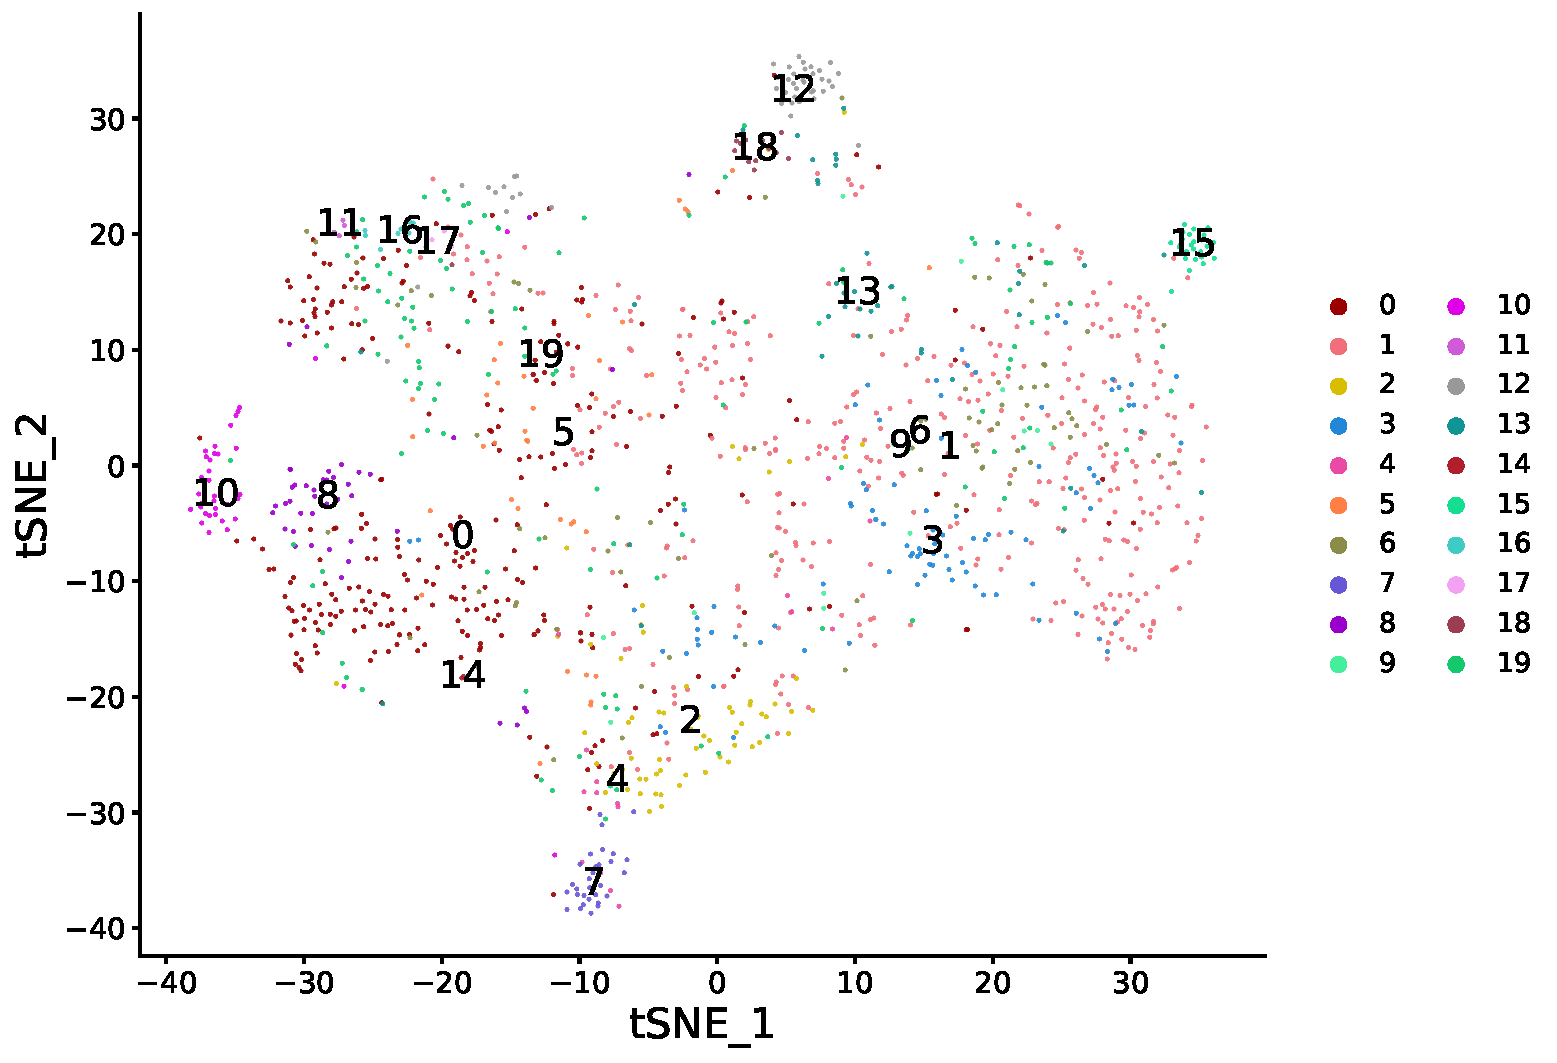
\includegraphics[width=0.23\textwidth]{fig_tsne_fedproto.pdf} &
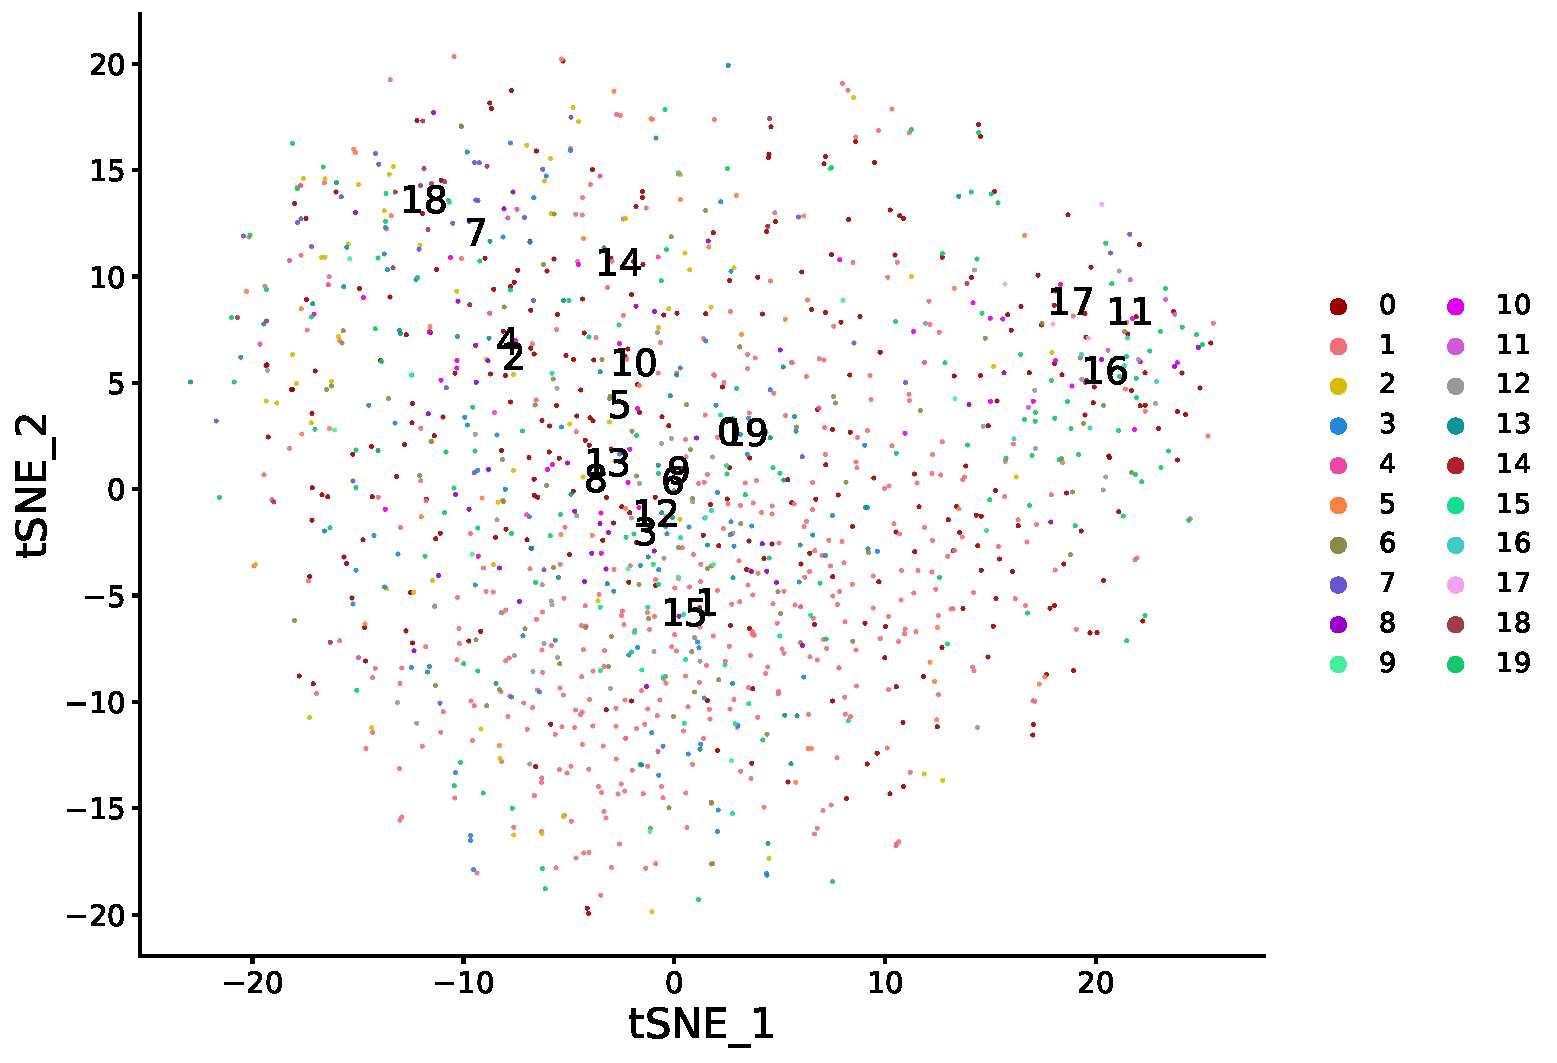
\includegraphics[width=0.23\textwidth]{fig_tsne_fedgmkd.pdf} \\
{\small (a) FedProto} & {\small (b) FedGMKD} \\
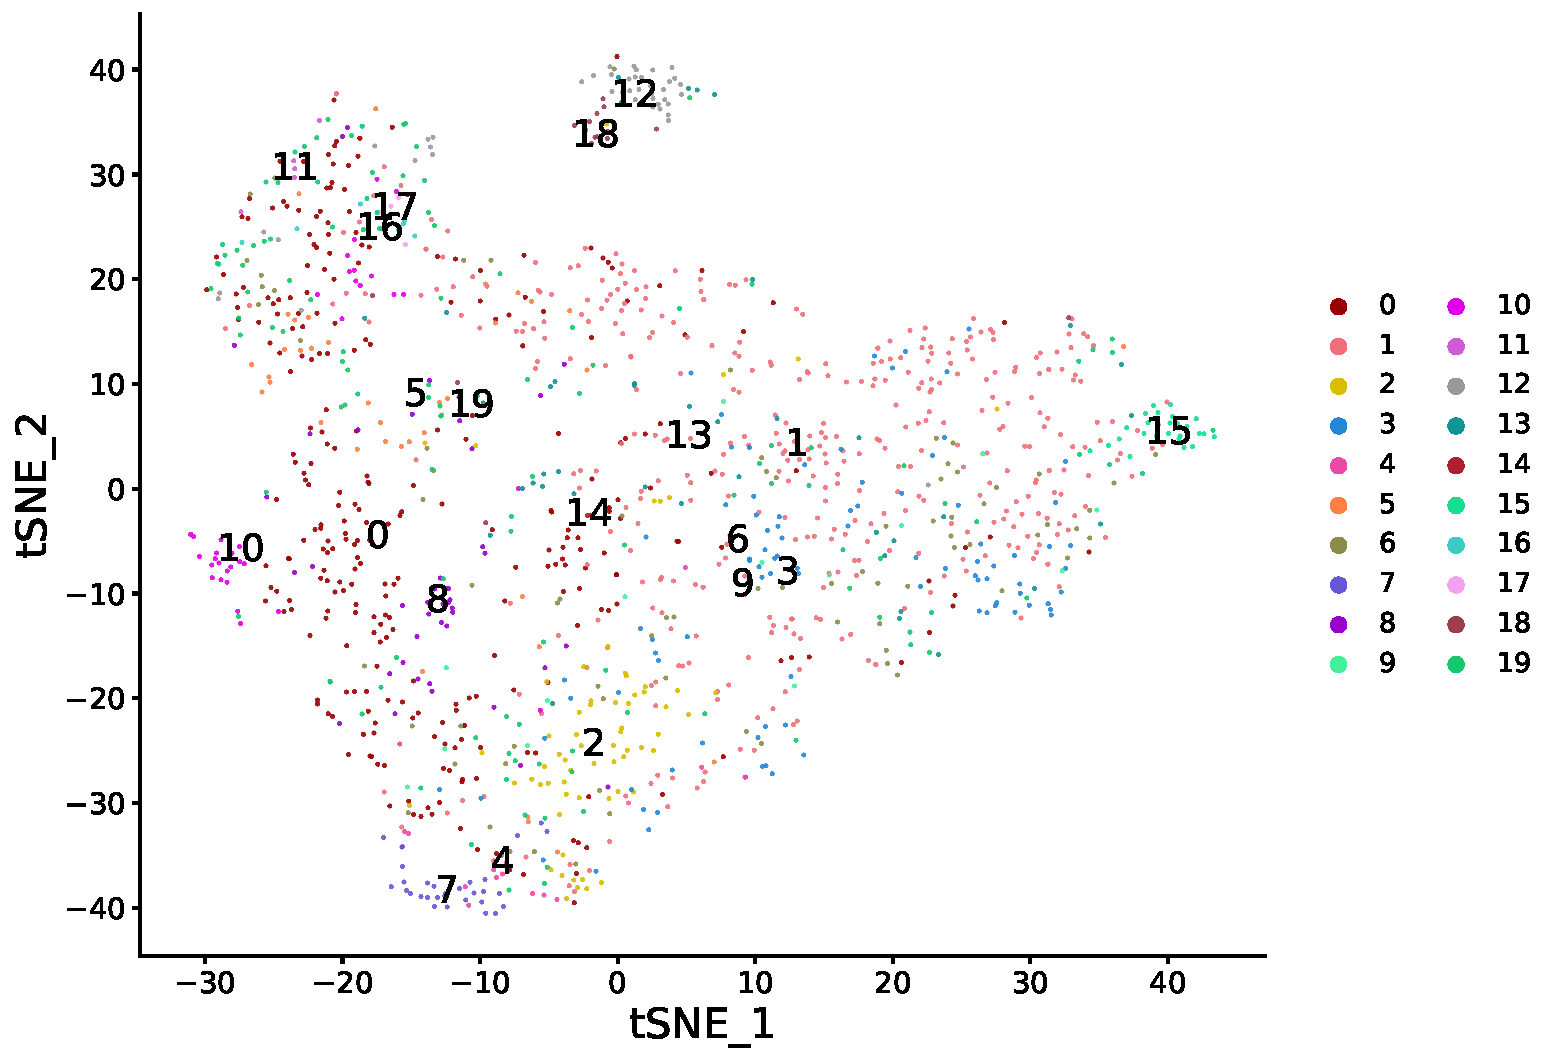
\includegraphics[width=0.23\textwidth]{fig_tsne_fedseproto.pdf} &
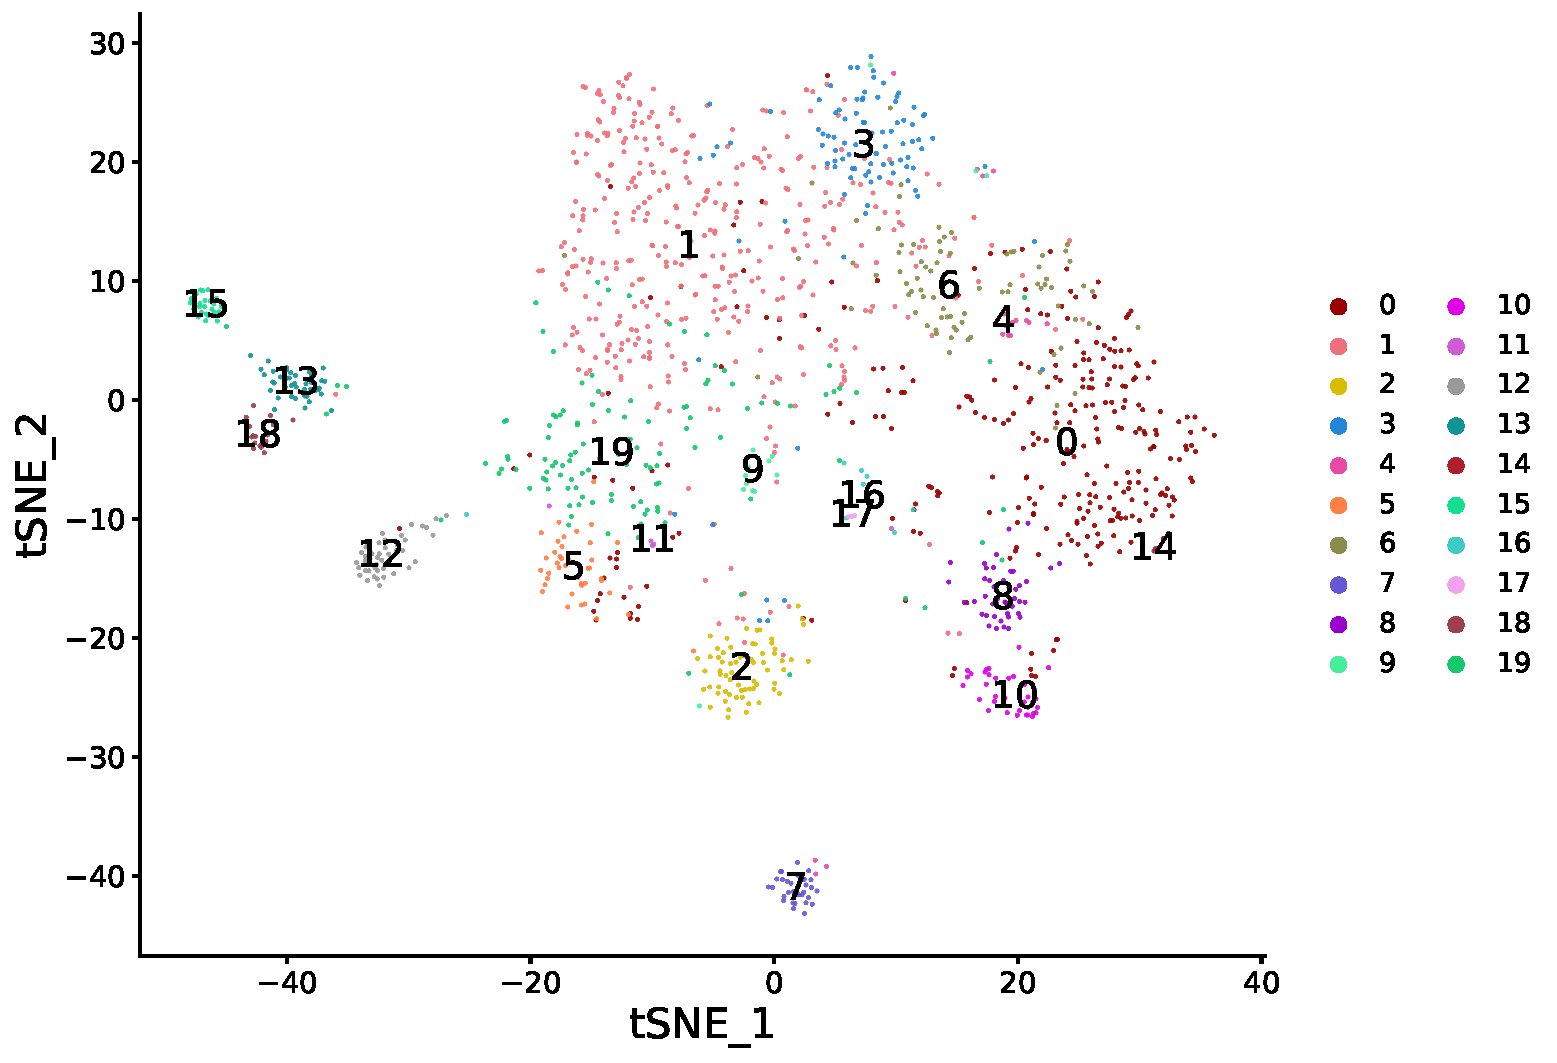
\includegraphics[width=0.23\textwidth]{fig_tsne_fedcop.pdf} \\
{\small (c) FedSeProto} & {\small (d) FedCoP (ours)} \\
\end{tabular}
\caption{t-SNE of sample embeddings on MuReD (20 classes; color = class). FedCoP exhibits structured layout where known co-occurring pathologies occupy adjacent regions, confirming the effect of $L_{co}$.}
\label{fig:tsne}
\end{figure}

Figure~\ref{fig:tsne} shows t-SNE embeddings on MuReD. In the three baselines, class clusters are scattered with no apparent structure governing relative positions. FedCoP exhibits a visibly more structured layout: co-occurring classes (e.g., diabetic retinopathy and macular edema) occupy adjacent regions. This is the geometric signature of $L_{co}$---by aligning prototype cosine Gram to $\Rhat$, the loss organizes embedding topology to reflect clinical comorbidity. The structure emerges despite no single client seeing all 20 classes ($\text{ways}{=}15$), corroborating Prop.~\ref{prop:estimation}(c).

\subsection{Ablations}
\label{sec:ablation}

We separately toggle each component: federated vs.\ local vs.\ no co-occurrence structure, $L_{co}$ loss, mean-field decoder, distributional vs.\ point prototypes, entropy regularizer, logit fusion ratio, distance metric, and temperature. All variants use the same backbone, split, and seed. Table~\ref{tab:ablation} summarizes key ablations on ChestX-ray14.

\begin{table}[t]
\centering
\caption{Key ablation results on ChestX-ray14. Full variant matrix in supplementary.}
\label{tab:ablation}
\footnotesize
\setlength{\tabcolsep}{3pt}
\begin{tabular}{lcccc}
\toprule
Variant & m-AUC & m-F1 & Ham. & Acc \\
\midrule
FedCoP (full)                  & \textbf{0.7053} & 0.2949 & \textbf{0.1956} & 0.9083 \\
~~--no co-occurrence ($\Rhat{=}I$) & 0.6938 & 0.2861 & 0.2112 & 0.8955 \\
~~--no $L_{co}$                 & 0.6981 & 0.2894 & 0.2038 & 0.9017 \\
~~--no MF decoder              & 0.7004 & 0.2911 & 0.2005 & 0.9048 \\
~~local $\Rhat$ (per-client)   & 0.6892 & 0.2803 & 0.2187 & 0.8901 \\
~~point prototypes             & 0.6965 & 0.2847 & 0.2089 & 0.8976 \\
~~no $L_{ent}$                 & 0.6944 & 0.2877 & 0.2091 & 0.8950 \\
\midrule
no $L_{co}$ + no MF decoder ($\Rhat$ unused) & 0.6841 & 0.2724 & 0.2245 & 0.8843 \\
\bottomrule
\end{tabular}
\end{table}

\noindent\textbf{Federated $\Rhat$ vs.\ local vs.\ none.} Removing $\Rhat$ entirely ($\Rhat{=}I$) drops macro-AUROC by 1.6\%. Using per-client local $\Rhat$ is \emph{worse} than using none (0.6892 vs.\ 0.6938), confirming Prop.~\ref{prop:estimation}(c): local estimates are biased and noisy under non-IID partitioning.

\noindent\textbf{Training-side $L_{co}$ vs.\ inference-side decoder.} Removing $L_{co}$ costs 1.0\% macro-AUROC; removing the decoder costs 0.7\%. Removing both (last row) costs 3.0\%, confirming they are complementary and not redundant.

\noindent\textbf{Distributional vs.\ point prototypes.} Switching to point prototypes drops 1.2\%---variance information matters for Bayesian fusion quality.

\noindent\textbf{Entropy regularizer.} Removing $L_{ent}$ drops 1.5\%, confirming that variance collapse silently degrades distributional prototypes.

\noindent\textbf{Full results.} The complete variant matrix (36 configurations, both datasets) is provided in the supplementary material, along with per-class AUROC breakdowns and analyses of logit fusion ratio $\alpha$, temperature $T$, and distance metric (Euclidean vs.\ Mahalanobis vs.\ cosine).

% =====================================================================
\section{Conclusion}

We argued that pathology co-occurrence is an intrinsically federated quantity, invisible to any single client that sees only a subset of classes and recoverable only by aggregation of label sufficient statistics. FedCoP estimates this structure federatedly and uses it on both sides of the pipeline: a structure loss aligns prototype geometry to the estimated correlation, and a mean-field decoder propagates evidence across co-occurring classes at inference. The theory establishes that the independent decoder is Bayes-optimal only under conditional independence and that the mean-field decoder is never worse, while the federated estimator is unbiased under participation reweighting and concentrates. Experiments on ChestX-ray14 and MuReD confirm consistent gains, and comprehensive ablations isolate each component's contribution.

Two limitations: $\Rhat$ approximates the residual correlation $\Sigmay$ rather than equaling it (shrinkage hedges this); and the non-recoverability argument assumes strict subset class supports (when supports overlap substantially, local estimates become informative and the federated gain narrows). Extending the estimator to the conditional regime and to streaming participation are natural next steps.

% =====================================================================
{
    \small
    \bibliographystyle{ieeenat_fullname}
    \bibliography{FedCoP_wacv}
}

\end{document}
